\providecommand{\main}{..}
\documentclass[\main/master.tex]{subfiles}
\begin{document}
\chapter{Theoretical background}\label{chapter:Theoretical background}
\section{Torsional pendulum}
\subsection{Torsional pendulum}
\begin{figure}[htbp]
	\centering
	\fbox{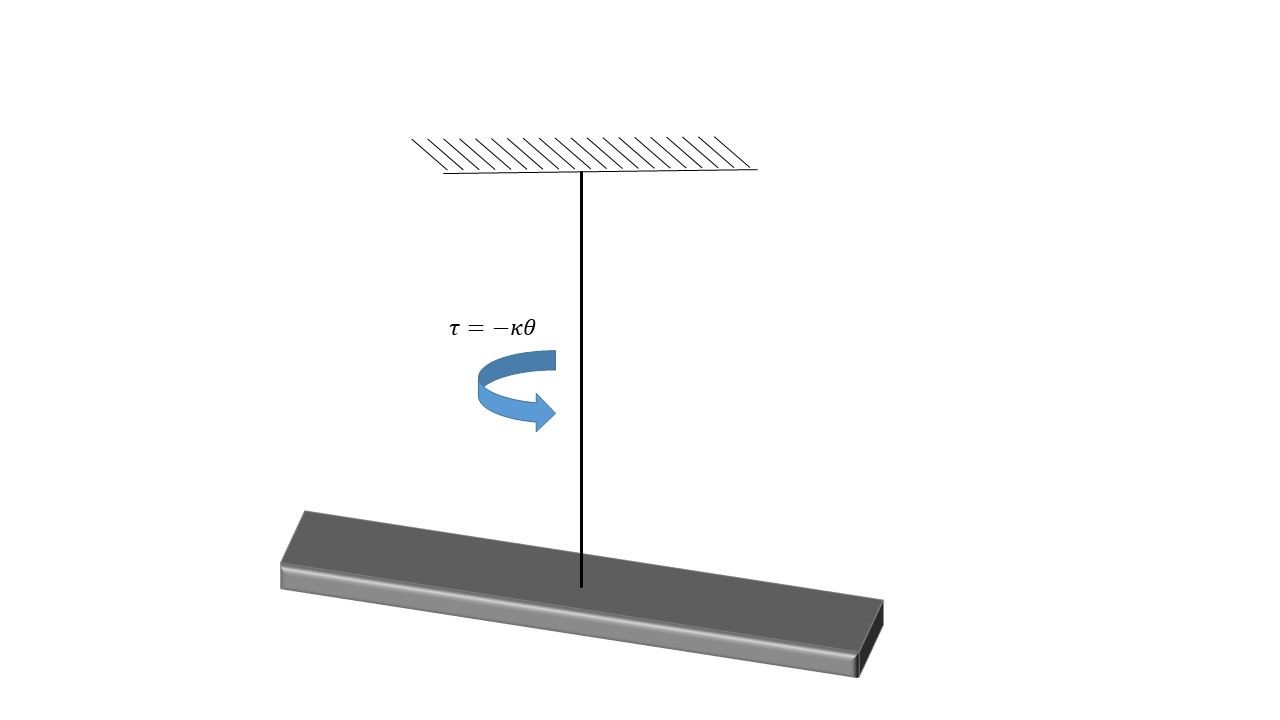
\includegraphics[scale=0.2]{\main/images/2 - theoretical background/torsion_pendulum_powerpoint.jpg}}
	\caption[Torsional pendulum]{A torsional pendulum}
	\label{fig:torsion_pendulum}
\end{figure}
\par\noindent
A torsional pendulum, shown in fig.~\ref{fig:torsion_pendulum}, is an oscillator made of a mass hung by a string from a fixed point allowing it to swing freely. When the mass is displaced from the equilibrium angle, the pendulum has a linear restoring torque, caused by the twisted string. 
\par\noindent
The restoring torque $\tau$, which is proportional to the string torsion coefficient $\kappa$, rotates the mass back to the equilibrium position:
\begin{equation}
\tau = -\kappa\cdot\theta     \label{eqn:hook law}
\end{equation}

\par\noindent
Assuming homogeneity of a circular string, the string torsion coefficient $\kappa$ can be estimated by:
\begin{equation}
\kappa = \frac{GJ}{h} = \frac{G}{h} \frac{\pi(\frac{d}{2})^4}{2}  = \frac{G}{h} \frac{\pi d^4}{32}   \label{eqn:torsion_coefficient_homogeneity}
\end{equation}
\par\noindent
Where $G$ is the material shear modulus, $J$ is the circular second moment of area ($Jzz$), $h$ is the string length and $d$ is the string diameter.
 


\subsection{Simple harmonic oscillator}
The harmonic oscillator is a second order system that, when displaced, experiences a linear restoring force proportional to the displacement from equilibrium. The torsional pendulum is an angular harmonic oscillator. However, it is equivalent to the linear case, where instead of velocity and force, one has angular velocity and torque.
\par\noindent
If the restoring torque $\tau$ is the only torque in action, then the oscillator is not driven oscillator, resulting in a simple harmonic motion:
\begin{equation}
\tau = -\kappa\theta  = I\ddot{\theta}   \label{eqn:undamped_motion_equation}
\end{equation}
\par\noindent
Where $I$ is the moment of inertia of the torsional pendulum. Solving eq.~\ref{eqn:undamped_motion_equation}, the restoring torque causes sinusoidal oscillations (simple harmonic motion) around the equilibrium angle:  
\begin{equation}
\theta(t) = \theta_{max}cos(\omega_0 t )    \label{eqn:undamped_motion_equation_solved}
\end{equation}
Where $\theta_{max}$ is the oscillations amplitude and $\omega_0$ is the natural resonant frequency of the oscillations.
\begin{equation}
\omega_0  = \frac{2\pi}{T} = \sqrt{\frac{\kappa}{I}}   \label{eqn:undamped_omega}
\end{equation}
\par\noindent
The time period of oscillation $T$ and $\omega_0$ are determined by the physical constants of the pendulum $\kappa$, $I$. Accordingly, the string torsion coefficient $\kappa$ could also be found empirically by finding the oscillations period $T$.


\subsection{Damped oscillator}
The system is a damped oscillator if there is also a damping torque $\tau = -b\dot{\theta}$. The damping torque is opposite to the oscillator's angular velocity $\dot{\theta}$, where $b$ is the oscillator damping coefficient. Thus, eq.~\ref{eqn:undamped_motion_equation} becomes:
\begin{equation}
\tau = -\kappa\theta - b\dot{\theta}  = I\ddot{\theta}   \label{eqn:damped_motion_equation}
\end{equation}
Eq.~\ref{eqn:damped_motion_equation} could be rewritten as:
\begin{equation}
\ddot{\theta} + 2\xi\omega_0\dot{\theta} + \omega_0^2\theta = 0   \label{eqn:damped_motion_equation_2}
\end{equation}
Where, $\xi$ is the oscillator damping ratio, which determines the oscillator damping type and damping time. The damping ratio is given by:
\begin{equation}
\xi = \frac{b}{2\sqrt{I\kappa}} 
\label{eqn:system damping ratio}
\end{equation}
The damping time $\tau$ is given by:
\begin{equation}
\tau = \frac{1}{\xi\omega_0} = \frac{1}{\frac{b}{2\sqrt{I\kappa}}\sqrt{\frac{\kappa}{I}} }= \frac{2I}{b}  \label{eqn:damping_time}
\end{equation}

\par\noindent
Solving eq.~\ref{eqn:damped_motion_equation_2}, the oscillator motion could be either undamped, overdamped, critically damped or underdamped, the motion is determined by the damping ratio value $\xi\geq 0$. 
%Assuming the boundaries $\theta(0) = \theta_{max}$ and $\dot{\theta}(0) = 0$, the oscillator motion is given by:
\par\noindent
When $\xi = 0$ the oscillator is undamped; there is no damping, leading to harmonic oscillations without decay:
\begin{equation}
\theta(t) = \theta_{max}cos(\omega_0 t )    \label{eqn:undamped_motion_equation_2}
\end{equation}
When $\xi < 1$ the oscillator is underdamped; amplitude of the oscillations decreases in time due to the damping friction while oscillating with a lower frequency due to the damping coefficient: 
\begin{equation}
\theta(t) = \theta_{max} e^{-\frac{t}{\tau}}cos(\sqrt{1-\xi^2}\omega_0 t ) =  \theta_{max} e^{-\frac{t}{\tau}}cos(\omega t )    \label{eqn:underdamped_motion_equation}
\end{equation}
When the damping coefficient is small enough, the frequency change is negligible, and can be approximated by:
\begin{equation}
\omega = \omega_0\sqrt{1-\xi^2}\approx\omega_0    \label{eqn:underdamped_frequency}
\end{equation}
\par\noindent
When $\xi = 1$ the oscillator is critically damped; due to high friction, the system cannot oscillate and it decays exponentially to the equilibrium position. As shown in eq.~\ref{eqn:system damping ratio}, choosing $b$ to be at the critical damping value would give the fastest return to the equilibrium position:
\begin{equation}
% A+B t (e^{-\frac{t}{\tau}}) 
\theta(t) = \theta_{max}(1+\frac{t}{\tau}) e^{-\frac{t}{\tau}}     \label{eqn:critically_damped_motion_equation}
\end{equation}
\par\noindent
When $\xi > 1$ the oscillator is overdamped; due to high friction, the system cannot oscillate and it decays exponentially to the equilibrium position. When defining $\xi'  = \frac{\xi}{\sqrt{\xi^2 - 1}}$ the motion is given by: 
\begin{equation}
\theta(t) = \frac{\theta_{max}}{2} [ (1-\xi')e^{-\frac{t}{\tau}(1+\frac{1}{\xi'})} +(1-\xi')e^{-\frac{t}{\tau}(1-\frac{1}{\xi'})} ]
\label{eqn:overdamped_motion_equation}
\end{equation}

\iffalse
\begin{equation}
\theta(t) = Ae^{-\frac{t}{\tau}(1+\sqrt{1-\frac{1}{\xi^2}})} + Be^{-\frac{t}{\tau}(1-\sqrt{1-\frac{1}{\xi^2}})}    \label{eqn:overdamped_motion_equation}
\end{equation}
\fi 
\par\noindent
Fig.~\ref{fig:damped_oscillators} shows a comparison of the different damping types oscillations:
\begin{figure}[htbp]
	\centering
	\fbox{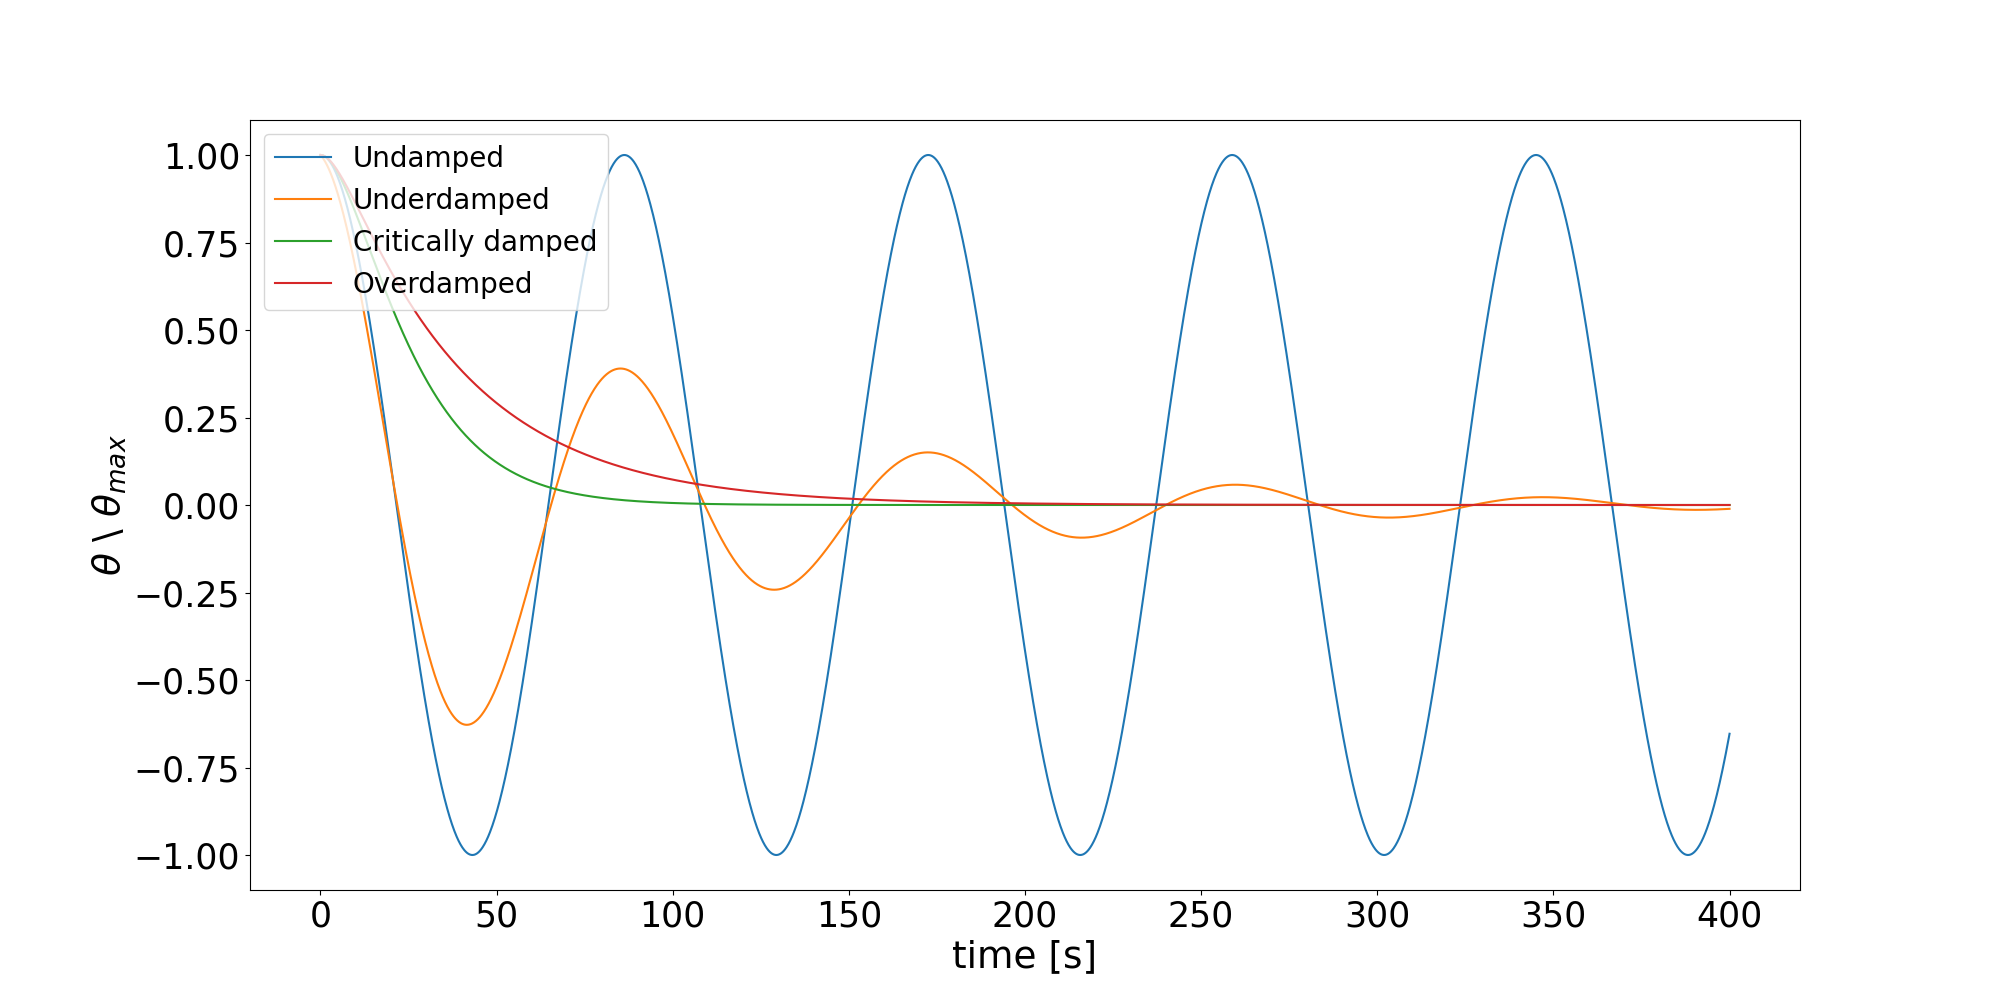
\includegraphics[scale=0.5]{\main/images/2 - theoretical background/damp.png}}
	\caption[Damped oscillators comparison]{Damped oscillators comparison}
	\label{fig:damped_oscillators}
\end{figure}
\FloatBarrier
\iffalse
https://ocw.mit.edu/courses/mathematics/18-03sc-differential-equations-fall-2011/unit-ii-second-order-constant-coefficient-linear-equations/damped-harmonic-oscillators/MIT18_03SCF11_s13_2text.pdf

https://www.sciencedirect.com/topics/engineering/underdamped-system#:~:text=When%20the%20damping%20ratio%20is%20between%200%20and%201%20(i.e.,is%20an%20exponential%20decay%20line.
\fi
\subsubsection{Driven oscillator}
If the damped oscillator system is further affected by an external time-dependent torque $\tau(t)$, the system is known as a driven oscillator, and its motion equation is:
\begin{equation}
\tau(t) -\kappa\theta - b\dot{\theta}  = I\ddot{\theta}   \label{eqn:driven_motion_equation}
\end{equation} 
Eq.~\ref{eqn:driven_motion_equation} could be rewritten as:
\begin{equation}
\ddot{\theta} + 2\xi\omega_0\dot{\theta} + \omega_0^2\theta = \frac{\tau(t)}{I}   \label{eqn:driven_motion_equation_2}
\end{equation}






\section{Gravity measurement}
\subsection{Gravitational field}
Newton's law of universal gravitation states that every mass $M$ attracts every other mass $m$ in the universe by force $F$ given by:
\begin{equation}
\overrightarrow{F}(r) = \frac{GMm}{r^2}\hat{r}    \label{eqn:gravitation_force}
\end{equation}
The force $F$ acts along the intersecting line, proportional to the product of the masses and inverse to the square of the distance $r$ between the centers. Since $G$ the gravitational constant, is very small, the force is very weak.
\par\noindent
The gravitational field $g$ of mass $M$ is defined as the force per unit mass, which is a vector field consisting, at every point, a vector pointing directly towards the mass. The magnitude of the field at every point is calculated by applying the universal law, given by: 
\begin{equation}
\overrightarrow{g}(r) = \frac{\overrightarrow{F}(r)}{m} = \frac{GM}{r^2}\hat{r}    \label{eqn:gravitation_field}
\end{equation}
\iffalse
\subsubsection{Field measurement}
\par\noindent
The field caused by a test mass $M$ at a specific point is calculated by measuring the gravitational force acting on a known mass $m$. In general, test mass $M$ is much larger than mass $m$, ensuring a negligible influence on the behavior of $M$.  
\fi
\subsection{Cavendish experiment}
\begin{figure}[htbp]
	\centering
	\fbox{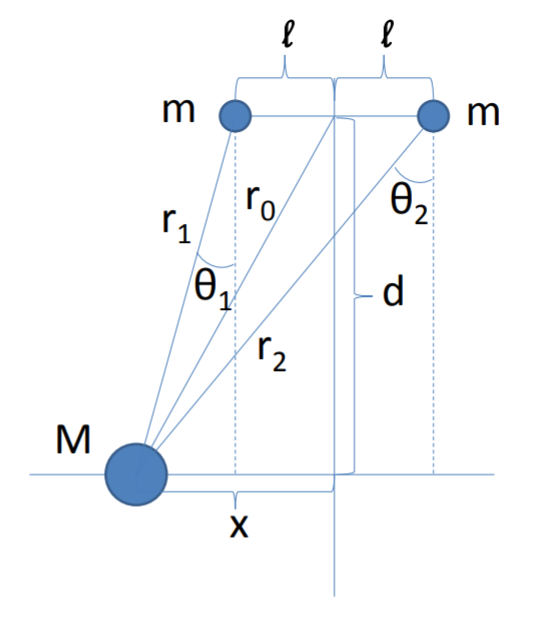
\includegraphics[scale=0.7]{\main/images/2 - theoretical background/Cavendish apparatus.PNG}}
	\caption[Cavendish apparatus]{Cavendish apparatus \cite{howell2019}}
	\label{fig:Cavendish apparatus}
\end{figure}
\FloatBarrier
\par\noindent
The Cavendish apparatus, shown in fig.~\ref{fig:Cavendish apparatus}, measures the gravitational force between masses. The apparatus is constructed by a torsional pendulum and a nearby test mass $M$, creating a net torque on the pendulum. 
\par\noindent
The pendulum can be assumed to consist of two masses $m$ connected by a rigid, massless thin rod, with length of $2l$, and a pivot point at distance $l$ from each mass. The moment of inertia $I$ of a torsional pendulum oscillating around the pivot is given by:
\begin{equation}
I = 2ml^2     \label{eqn:moment_inertia}
\end{equation} 
The mass $M$, located at distance $r_0$ from the pivot point attracts the two masses and creates torques. The net gravitational torque $\tau_g$ for a balanced torsional pendulum is the sum of two inverse, nearly counterbalancing, gravitational torques, one from each mass $m$:
\begin{equation}
\tau_g = l \cdot F(r_1) \cdot cos\theta_1 - l \cdot F(r_2) \cdot cos\theta_2 = l d GmM(\frac{1}{r_1^3} - \frac{1}{r_2^3})     \label{eqn:net_gravitation_torque}
\end{equation}
Defining the function $h(l)$:
\begin{equation}
h(l) = \frac{1}{(d^2 +(x-l)^2)^{3/2}} \label{eqn:gravitation torque func}
\end{equation}
Where $h(l) = \frac{1}{r_1^3},\quad	h(-l) = \frac{1}{r_2^3},\quad	h(0) = \frac{1}{r_0^3}$, and the derivative is: $h'(0) = \frac{3x}{r_0^5}$. Since $l<<d,x,r_0$ one can approximate:
\begin{equation}
h(l)-h(-l)\approx h'(0)\cdot 2l = \frac{6lx}{r_0^5}\label{eqn:approximation}
\end{equation}
According to eq.~\ref{eqn:net_gravitation_torque}, the net torque is proportional to the difference $h(l)-h(-l)$:
\begin{equation}
\tau_g = l d GmM[h(l)-h(-l)]\approx \frac{6l^2GmMxd} {r_0^5} = \frac{6l^2GmM sin\theta cos\theta}{r_0^3}      
\label{eqn:net_gravitation_torque_approx}
\end{equation}
Where $\theta$ is the tilt angle of the torsional pendulum and approximately $\theta_1 \approx \theta_2 = \theta$.
\subsubsection{Simple harmonic oscillator}
Assuming no friction or other damping force (simple harmonic motion) when a test mass $M$ is introduced, there are two sources of torque in the system; the net torque caused by the gravitational force $\tau_g$ (eq.~\ref{eqn:net_gravitation_torque_approx}), and a restoring torque at the opposite direction caused by the wire torsion (eq.~\ref{eqn:hook law},eq.~\ref{eqn:undamped_omega}):
\begin{equation}
\tau = \tau_g - \kappa\theta = \tau_g - (I\omega_0^2)\theta    \label{eqn:gravitation_torque}
\end{equation}
\par\noindent
At equilibrium, the two sources of torque cancel each other out:
\begin{equation}
\tau_g =  \kappa\theta    \label{eqn:gravitation_torque_equilibrium}
\end{equation}
Accordingly, with moment of inertia $I$ (eq.~\ref{eqn:moment_inertia}) the average tilt angle  $\overline{\theta}$ is given by:
\begin{equation}
\overline{\theta} = \frac{\tau_g}{\kappa} =\frac{\tau_g}{I\omega_0^2}  \approx \frac{6l^2GmMcos\theta sin\theta}{2ml^2 (\frac{2\pi}{T})^2 r_0^3} \approx \frac{3GT^2cos\theta sin\theta}{4\pi^2 } \cdot \frac{M}{r_0^3}  \label{eqn:theta average}
\end{equation} 

\par\noindent
The pendulum equilibrium angle is proportional to the square of the period's length $T$, the pendulum length $l$ as well as the masses $m$ are dropped out, indicating that short and light weight sensors work well as larger ones, as long as their periods are the same.
\par\noindent
According to eq.~\ref{eqn:theta average}, by accurate angle measurement, the gravitational field could be estimated.
 

\subsection{Gravity sensing}
The field at a specific point is the superposition of multiple fields, caused by any mass in space $M$ acting on the mass $m$ located at that point. Measuring the gravitational field caused by a specific test mass $M$ accurately with known mass $m$, the test mass $M$ weight or its distance could be estimated. In order to filter out the other gravitational fields caused by masses around, one measures the difference from a baseline state.
\par\noindent
Usually the measurement is based on measuring oscillation frequency. The test mass oscillates in different frequencies. The masses around that do not move, are filtered out.
\par\noindent
The sensor's tilt angle caused by the gravitational field is measured at each frequency, measuring the energy spectral density $[\frac{rad}{\sqrt{Hz}}]$ of the sensor.
In the measurement system different noises have different frequencies. By integrating over long periods, measurement noises are reduced. The signal to noise ratio (SNR) is the limiting factor for the sensitivity of a measuring system. In higher frequencies the integration is faster, causing less noises and higher SNR.
The dependency of the SNR on frequency causes difficulties when measuring gravitational fields at low frequencies.
\par\noindent
This limitation is a significant challenge while designing gravimetric sensors for low frequencies.

\subsubsection{The shot noise limit}
The shot noise is a fundamental quantum physical phenomenon in which the power of an optical signal fluctuates due to fluctuations in the number of photons in the signal. The power of an optical signal $p_{signal}$ is:
\begin{equation}
p_{signal} = N h \nu   \label{eqn:signal_power}
\end{equation}
Where $N$ is the number of photons, $h$ is the Planck constant and $\nu$ is the photon frequency. Since the shot noise is a Poisson process, the shot noise power $p_{shot}$ can be calculated as the root mean square (RMS) of the current fluctuations power:
\begin{equation}
p_{shot} = \sqrt{p}    \label{eqn:shot_power}
\end{equation}
An optical measurement system with coherent light can not measure a signal smaller than its shot noise, the SNR of a shot noise limited system is:
\begin{equation}
SNR = \frac{p_{signal}}{p_{shot}} =\frac{N}{\sqrt{N}} = \sqrt{N}    \label{eqn:shot_noise}
\end{equation}
However, while other system noises are higher than the shot noise limit, reducing noises and averaging the time integration can provide higher accuracy and better measurement results. 
\section{Radiation-pressure}
Radiation-pressure is the pressure of a light beam on the surface due to momentum exchange with the electromagnetic field. The momentum exchange may occur with light at any wavelength which is absorbed, reflected, or emitted by the surface. The pressure causes a force on the surface, although this force is usually insignificant.  
\par\noindent
The radiation-pressure force depends on the surface angle relative to the electromagnetic field propagating direction, as well as the surface reflectance and absorbance, and the power of light hitting the surface $\Theta_i$ (radiant flux, measured in watts). Assuming that the beam is focused tightly enough that variation over the surface is negligible, the incident radiation pressure is given by:
\begin{equation}
P_{incident} = \frac{\frac{\Theta_i}{A}cos^2(\alpha)}{c} = \frac{\eta\cdot \Theta_{source}\cdot cos^2(\alpha)}{{A\cdot c}} \label{eqn:radiation_pressure}
\end{equation}
Where $\alpha$ is the field angle, compared to the surface area $A$, $c$ is the speed of light and $\eta$ is the coupling efficiency due to light losses. The light losses are caused by the light beam passing through light transmitters (such as light guide or fiber), and size difference between the light beam size and the target size. 
\par\noindent
When the light field direction is perpendicular to the surface the radiation pressure is:
\begin{equation}
P_{incident} = \frac{\eta\Theta_{source}}{{Ac}} \label{eqn:radiation_pressure_perpendicular}
\end{equation}
\par\noindent
For a reflective material with reflectivity $R$, the radiation force is:
\begin{equation}
F = P_{total}\cdot A = (P_{incident}+P_{reflected})\cdot A = P_{incident}(1+R)A \label{eqn:radiation_force}
\end{equation}
For a material with high reflectivity, $R\approx 1$:
\begin{equation}
F \approx 2P_{incident}A = \frac{2\eta\Theta_{source}}{{c}}\cdot \frac{A}{A} \label{eqn:radiation_force_reflective}
\end{equation}
Thus:
\begin{equation}
F \approx \frac{2\eta\Theta_{source}}{{c}} \label{eqn:radiation_force_power}
\end{equation}

\section{Pressure and environment affects}
\subsection{Ideal gas}
An ideal gas is a theoretical gas composed of many randomly moving gas particles that are not having interparticle interactions. The ideal gas law is given by:
\begin{equation}
PV = nRT = (n N_A) k_B T = N k_B T  \label{eqn:ideal-gasses}
\end{equation}
Where $P$ is the gas pressure, $V$ is the medium's volume, $R$ is the ideal gas constant, $T$ is the temperature and $k_B$ is the Boltzmann constant. The number of particles $N$ is a product of the number of moles $n$ and the Avogadro constant $N_A$. For an ideal gas the density $\rho$ is given by:
\begin{equation}
\rho(P) = \frac{MP}{RT}     \label{eqn:ideal density}
\end{equation}
Where $M$ is the gas particles molar mass. For a diluted ideal gas the viscosity $\mu$ is given by:
\begin{equation}
\mu(P) = \alpha l \rho \sqrt{\frac{2\pi k_B  T}{\pi m}}      \label{eqn:viscosity}
\end{equation}
Where $\alpha$ is a numerical constant, $l$ is the mean free path of the gas particles and $m$ is the molecular mass. 

\subsection{Friction}
The drag force $F_{drag}$ is the friction caused by gas resistance, which is dependent on the relative velocity (the gas flow velocity) $v$ between the gas and the object. At higher pressures, when the gas is having a turbulent flow, the drag is proportional to the square of the velocity:
\begin{equation}
F_{drag} = -\frac{1}{2}\rho C_d A \cdot v^2 = -b\cdot v^2 
\label{eqn:drag force}
\end{equation}
Where $C_d$ is the drag coefficient and $b$ is the drag force proportionality factor. When pressure decreases the gas is having a laminar flow, and the drag force is given by Stokes' law:
\begin{equation}
F_{drag} = -6\pi\mu r\cdot v = -b\cdot v
\label{eqn:drag force}
\end{equation}
Where $r$ is the radius of the area cross section. For ideal gas both the density and viscosity are pressure dependent, and decrease with pressure. Due to the pressure dependency of the drag force, decreased pressure results with lower drag force.

\subsection{Brownian motion}
\subsubsection{Brownian energy}
Brownian motion is the pattern of random particles' fluctuations at fluid or gas phases, a random walk with no preferential direction of flow. This pattern happens at thermal equilibrium in a given temperature (on average there is no linear and angular momentum). The Maxwell-Boltzmann distribution of molecular velocity is given by:
\begin{equation}
f(v) = 4\pi(\frac{m}{2 \pi k_B T})^{3/2}\cdot v^2\cdot exp(\frac{-mv^2}{2k_BT})     \label{eqn:Maxwell_Boltzmann}
\end{equation} 
\par\noindent 
Thus, the average kinetic energy for a gas particle is: 
\begin{equation}
<E_k>=<\frac{mv^2}{2}> = \int_{0}^{\infty}\frac{mv^2}{2}f(v)dv =  \frac{3k_BT}{2}    \label{eqn:average kinetic}
\end{equation}
\par\noindent
The total Brownian motion energy is:
\begin{equation}
E_k = N<E_k> =\frac{3}{2}N k_B T = \frac{3}{2}PV    \label{eqn:total_kinetic}
\end{equation}
\par\noindent
Eq.~\ref{eqn:total_kinetic} shows that the Brownian motion energy is proportional to the number of gas particles inside the medium. Reducing the gas pressure, which reduces the number of gas particles results In a reduction of the total Brownian motion energy. 
\subsubsection{Energy coupling}
There is thermal energy coupling from the environment on the sides of the medium, phonons are penetrating and passing energy to gas particles inside the medium. It can be shown that for an ideal gas with specific heat capacity $c_v$, the heat flow propagation distance is $\Delta x ^2  = \frac{1}{3} l^2 $, and the thermal conductivity $\lambda$ is given by:
\begin{equation}
\lambda  = \frac{l}{3}\rho c_v v    \label{eqn:heat conduction coefficient}
\end{equation}
It can be shown from eq.~\ref{eqn:heat conduction}, that the average gas flow velocity $v$ is given by:
\begin{equation}
v =\sqrt{\frac{3k_B T}{m}}=\sqrt{\frac{3 T k_B N_A}{M}} =  \sqrt{\frac{3RT}{M}}   
\label{eqn:flow velocity}
\end{equation}
The thermal coupling power from the environment $p$ is given by Fourier's law of heat conduction:
\begin{equation}
p =  \lambda A \frac{\Delta T}{\Delta x} =\frac{l}{3} \frac{MP}{RT} c_v v A \frac{\Delta T}{\sqrt{\frac{1}{3} l^2 }} = \frac{M P c_v  A \Delta T}{\sqrt{3}RT} \sqrt{\frac{3RT}{M}} =   \sqrt{\frac{M}{RT}} c_v  A P  \Delta T 
\label{eqn:heat conduction}
\end{equation}
Eq.~\ref{eqn:heat conduction} shows that the thermal coupling power is proportional to the to the temperature difference $\Delta T$ and the gas pressure.
%https://www.tec-science.com/thermodynamics/heat/thermal-conduction-in-solids/
\iffalse
\subsubsection{Classical harmonic oscillators and equipartition of energy}
The Hamiltonian $H$ of a simple harmonic oscillator is:
\begin{equation}
H(p,x) = \frac{p^2}{2m}+\frac{1}{2}\kappa x^2
\label{eqn:Hamiltonian}
\end{equation}
The simple harmonic oscillator has a momentum $p$ and position $x$, which is one degree of freedom. For a classical continuous system with one degree of freedom the partition function $Z$ is:
\begin{equation}
Z = \frac{1}{h}\int_{-\infty}^{\infty}exp(-\frac{\kappa x^2}{2}\cdot \beta)dx \int_{-\infty}^{\infty} exp(-\frac{p^2}{2m}\cdot \beta)dp = 
\frac{1}{h} \sqrt{\frac{2\pi m}{\beta}} \sqrt{\frac{2\pi }{\kappa\beta} } = \frac{1}{\beta\hslash\omega}
\label{eqn:partition function}
\end{equation}
Where $\beta = \frac{1}{k_B T}$ is the thermodynamic beta. the thermodynamic energy of the oscillator is : 
\begin{equation}
E = -\frac{\partial}{\partial\beta}lnZ = -\frac{\partial}{\partial\beta}\frac{1}{\beta\hslash\omega} = \frac{1}{\beta}  = k_B T
\label{eqn:thermodynamic energy}
\end{equation}
The mean energy $E$ of an oscillator in equilibrium with a heat bath at temperature $T$, when heat bath is composed of ideal gas:
\begin{equation}
E = k_B T = k_B\frac{PV}{N k_B} = \frac{PV}{N}
\label{eqn:Brownian uncertainty}
\end{equation}
According to the equipartition theorem, the average energy per degree of freedom is half the thermal
energy:

The Brownian motion kinetic energy is proportional to the temperature. The noise of quantum uncertainty due to Brownian motion at a given temperature is: 
\begin{equation}
\frac{1}{2}\kappa (\delta\theta)^2= \frac{1}{2}k_BT  \label{eqn:Brownian uncertainty}
\end{equation}
\begin{equation}
\delta\theta = \sqrt{\frac{k_B T}{\kappa}}  \label{eqn:Brownian uncertainty 2}
\end{equation}
\fi
\subsection{Radiative cooling}
Radiative cooling is a phenomenon in which a black body loses heat by thermal radiation to remain in thermal equilibrium at constant temperature $T$. The thermal radiation power $p_{emit}$ over all frequencies is given by the Stefan–Boltzmann law:
\begin{equation}
p_{emit} = \sigma\epsilon A T^4  \label{eqn: Stefan–Boltzmann law}
\end{equation}
Where $\sigma$ is the Stefan–Boltzmann constant, and the emissivity $\epsilon$ is a value which defines how close the black body to an ideal black body. The net absorbed power $p$ is given by: 
\begin{equation}
p = p_{absorb}-p_{emit} = \sigma\epsilon A (T_0^4-T^4)  \label{eqn: Stefan–Boltzmann power}
\end{equation}
Where $T_0$ is the environment temperature and $T$ is the black body temperature.  
\subsection{Acoustic wave}
Acoustic waves are adiabatic compression and decompression waves propagating through a material. The wave equation of one dimension acoustic wave:
\begin{equation}
P = P_0 cos(\omega t -k x)       \label{eqn:acoustic_pressure}
\end{equation}
\par\noindent
Where $P$ is the actual pressure, $P_0$ is the average pressure, $k$ is the acoustic wave number and $\omega$ is the wave angular frequency. Acoustic energy is carried by the acoustic waves, the acoustic power $p$ is the rate acoustic energy is emitted, given by:
\begin{equation}
p = AP u  = A P\sqrt{\frac{K_s}{\rho}}     \label{eqn:acoustic_intensity}
\end{equation}
Where $u$ is the material acoustic velocity and $K_s$ is the modulus of bulk elasticity for gases. When the material pressure is reduced, the acoustic pressure is lower and less power is carried.


\subsection{Vacuum quality}
\subsubsection{Leak rate}
At any vacuum system, some gas slowly leaks over time and increases the gas pressure if not pumped out, the leak rate $Q_L$ is given by: 
\begin{equation}
Q_L = \frac{\Delta P\cdot V}{\Delta t}  \label{eqn:leak rate}
\end{equation}
Where $\Delta P$ is the difference between the internal pressure and the external pressure, causing a sustained pressure increase over time $\Delta t$ for a given volume.

%The leak rate could also prevent the system from reaching initial low pressure, since at some point the leakage would be equal to the pumping rate.
%There is also a diffusion rate of gas molecules, such as helium, which is insignificant when pressure is above $10^{-9}$ [Torr] (vacuum lower than high vacuum). 

\subsubsection{Outgassing}
\par\noindent
At low pressures, there are more gas molecules (primarily water) bound to the chamber surfaces than floating in the chamber. When pressure is below vapor-pressure there is a desorption of the gas molecules from the material. Outgassing is the desorption rate $Q_{des}$ which over time increases the pressure:
\begin{equation}
Q_{des} = q_{des} A\frac{t_0}{t}  \label{eqn:desorption rate}
\end{equation}
Where $A$ is the surface area, and $q_{des}$ is the desorption density, which is area dependent. The desorption rate $Q_{des}$ produces a gas yield that declines over time. It could be assumed that after a given time $t_0$, typically one hour, the pressure increase is linear over time.
\par\noindent
The outgassing is minimized by selecting low vapor-pressure materials such as stainless steel and glass. Since water is a significant source of outgassing, the outgassing is usually minimized by baking the chamber at high temperatures while having the vacuum pump running (bake-out).
\subsection{Faraday cage}
\par\noindent
Faraday cage is a cage made by continuous covering of a conductive material used to block external electromagnetic fields. The external electrical fields cause an electric charge distribution in the conductive cage without passing inside. Electric current decays exponentially with depth through the material. The material skin depth $\delta$ defines the magnetic field's penetration depth, given by:
\begin{equation}
\delta = \sqrt{\frac{2\rho}{(2\pi f)(\mu)} }    \label{eqn:skin depth}
\end{equation}
Where $\rho$ is the material electric resistivity, $\mu$ the magnetic permeability and $f$ is the frequency of the magnetic field.


\section{Proportional–integral–derivative (PID) controller}
\begin{figure}[htbp]
	\centering
	\fbox{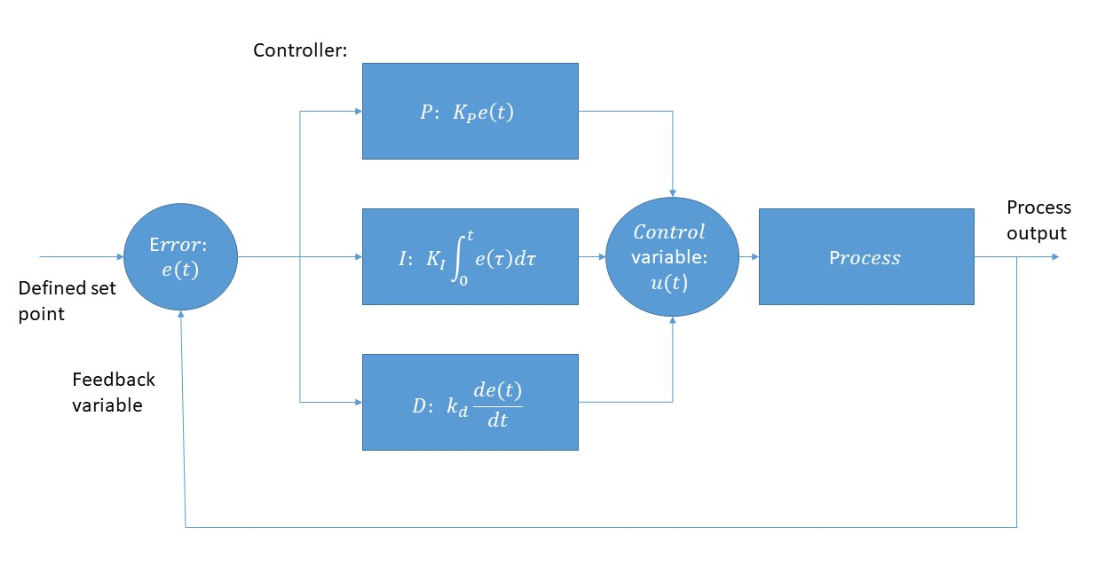
\includegraphics[scale=0.4]{\main/images/2 - theoretical background/pid_diagram_powerpoint.jpg}}
	\caption[PID controller block diagram]{PID controller block diagram}
	\label{fig:PID_scheme}
\end{figure}
\FloatBarrier
\par\noindent
Proportional–integral–derivative (PID) controller, shown in fig.~\ref{fig:PID_scheme}, is a feedback based control system. The control loop is used for time continuous control of a process, so the process output is close to a defined set point.
\par\noindent
PID controller continuously calculates error value, which is the difference of the process output from the defined set point. The feedback applies an external correction to the process, called control variable. The control variable is based on a gain to the error of proportional $P$, integral $I$ and derivative $D$. Proper tuning of a PID enables an accurate automated correction to a controlled process. The PID concept is used widely in applications requiring accurate automated control.

\par\noindent
The error and its integral and derivate are calculated continuously. The control has three tuning parameters; $K_P, K_I, K_D$, the feed back correction is modulated by the tuning parameters' value. Each parameter is assigned to a gain (P-I-D). The response (control variable) is a weighted sum of the control terms. Over time the controller attempts to minimize the error $e(t)$ by adjusting the control variable $u(t)$, which is the PID output:
\par\noindent

\begin{equation}
u(t) = K_P e(t)+K_I\int_{0}^{t}e(\tau)d\tau+K_D\frac{de(t)}{dt}   \label{eqn:PID response}
\end{equation}

\noindent
$P$ is proportional to the current error value $e(t)$. When error is large and positive, proportional output would be proportionately large and positive.
\par\noindent
$I$ is proportional to past error value's integration. The response of the cumulative value could eliminate residual errors, such as signal offset.
\par\noindent
$D$ is proportional to error current change rate, by calculating the derivative. The response of the change rate could eliminate more rapid changes.
\par\noindent
The optimal control function is achieved by balancing the responses. The tuning constants depend on the characteristics of the specific process. The response must be tuned for each control application.  

\end{document}







